\chapter{Background}
\label{chapter:background} 

This section introduces the theoretical background of the thesis. First the l

\section{Limited Liability Housing Company}

In this chapter the regime of limited liability housing company is presented and the operation of it is described in order to provide background information. First the basic concept is explained, then the responsibilities and operation of the limited liability housing company is presented.

Limited liability housing company is a type of limited liability company whose purpose is to own and control one or multiple building or a part of it where over the half of the combined floor surface area of the apartment or apartments is designated in the articles of association to be possessed by the shareholders and to be used as residential apartments \parencite{LLHA:2}. To put it simple, the company owns the property and the share capital is divided into shares. For the shareholders, these shares then give a right of possession to a specific apartment. \parencite{Lujanen:2017}. So, when a person buys an apartment in a limited liability housing company, she become the shareholder of the bought apartment \parencite{YIT}.

In Finland about 2,7 million people are living in approximately 88 000 limited liability housing companies \parencite{REMF, Stats}. This limited liability housing company regime is an unique setting compared to other countries and it is dominant form of ownership in multi-apartment buildings in Finland \parencite{Lujanen:2017}. The operation of the limited liability company is regulated in the Finnish law and the articles of association contains the internal law and order of the specific housing company \parencite{YIT}. In practice, the limited liability housing company takes care of the real estates and buildings to which it controls \parencite{LLHA:2}. 

\subsection{The Division of Responsibilities}

Limited liability housing company is led by the board and deputy landlord and their job is to act in a way that advances the company's interest \parencite{LLHA:2}. However, this does not mean that the people who are in the board should have expertise in the real estate field. So, the people working in the board are mostly laypersons which should be considered inside the board as well as among the shareholders. \parencite{Hallintotapa:2017}

The highest decision-making body is the shareholder's meeting which is held once a year. In a shareholder's meeting every shareholder has a right to vote. Shareholders one of the most important responsibility is to decide who will be in the board of the limited liability housing company. The Table~\ref{table:responsibilities} presents the actors who form the limited liability housing company and their responsibilities in addition to the previously mentioned. \parencite{RantanenViiala:2015} 

\begin{table}
\begin{tabular}{|p{2.5cm}|p{2.5cm}|p{6.4cm}|} 
\hline % The line on top of the table
\textbf{Organ} & \textbf{Chooser}  & \textbf{Responsibilities} \\ 
\hline 
Shareholder's meeting & Formed by all shareholders, not chosen & Shareholder's meeting decide on financial statement, maintenance fee, loans and major overhauls. Shareholder's meeting chooses the board members and gives the freedom of responsibility for the board members and the deputy landlord. In addition they chooses the auditor.\\ 
\hline
Board & Shareholder's meeting & The board chooses the deputy landlord, if the board do not take care of the real estate management by themselves. Board accepts the agreements and oversees the finance. Additionally the board makes a five year plan which covers the needed renovations and repairs. The board also presents the renovations done previously.\\
\hline
Deputy landlord & Board & Deputy landlord's responsibility is to take care of the daily operations of the limited liability housing company. Deputy landlord executes the decisions which the board has made. In addition deputy landlord prepares the board meetings and act as a secretary.\\
\hline
Service company & Board & Service company operates under deputy landlord and they do all tasks agreed on the agreements, for example cleaning of the public spaces.\\
\hline
Auditor & Shareholder's meeting & Auditor checks the company's accounts and the legality of the government. Auditor is responsible to report the status for the shareholder's meeting.\\
\hline
\end{tabular} % for really simple tables, you can just use tabular
% You can place the caption either below (like here) or above the table
\caption{Limited liability housing company's organs and their responsibilities. \parencite{RantanenViiala:2015}}
% Place the label just after the caption to make the link work
\label{table:responsibilities}
\end{table} % table makes a floating object with a title

The shareholder's meeting is a place where the shareholders, board members and the deputy landlord meet each other and the meeting provides a good place for discussions and questions \parencite{Hallintotapa:2017}. The decision making in a shareholder's meeting happens usually with the majority decision, which means that the suggestion which has over half of the votes is the final decision. If the voting is related to person, the one who receives most of the votes gets elected. In tie situation the chairperson makes the decision, if the voting is not related to electing a person. \parencite{RantanenViiala:2015}

In the shareholder's meeting the housing board's responsibility is to present the scope of the maintenance actions to be done in the limited liability housing company. This scope is then decided in the meeting. \parencite{RantanenViiala:2015} Based on the \textcite{LLHA:2} the board requires shareholder's meeting's decision to proceed with actions which are considering the size and operation of the company unusual or far-reaching, affecting essentially to the use of the shareholder's apartment or affecting essentially to the obligation to pay maintenance fee or to other expenses which are caused by the use of the shareholder's possessed apartment.

The role of the deputy landlord is similar to the managing director in a limited liability company since it is the deputy landlord's responsibility to take care of the daily administration.  Additionally, deputy landlord puts in action the decisions made by the housing board and takes care that the accounting is done properly according to the law. \parencite{Sarekoski:2015}

\section{Energy Industry in Finland}

This chapter focuses on the energy industry in Finland and how digitalization is affecting the industry and what it enables. Based on \textcite{Energiateollisuus:2018} energy industry is facing a time when customers role is changing towards the direction where they have more opportunities to influence the whole industry.

In Finland there are around 100 district heating companies which are responsible for heat distribution, sale and production. Most of these companies are owned by the municipalities. \parencite{Energyindustry:2019,Poyry:2018} Based on the statistics made by \textcite{Energyindustrygraphs:2018} 46 \% of apartment buildings are part of the district heating network which means that 2,92 million residents are living in apartments which are heated with district heating.

A study was done by \textcite{Deloitte} to find out how digitalization will change energy industry and what it will allow for the energy companies and for the customers. It was stated that digitalization is changing the business models and creating new services and products as well as forming new kind of customer experience. In addition the needs, expectations and hopes of the customers are driving the change in the energy industry. Energy efficiency is increasing and new alternative heating forms are becoming more popular, which are changing the current situation as well. \parencite{Energiateollisuus:2018}

According to the vision statement made by \textcite{Energiateollisuus:2018} Finland has the leader's role in reducing emissions, increasing renewable energy usage and in the use of combined heat and power as well as in district heating. Moreover, the prices are very competitive and the operational reliability is on it's own level. In addition digitalization allows the energy industry to be more efficient with lower expenses \parencite{Tekes:2017}.

According to the analyze made by \textcite{Deloitte} digitalization offers opportunities for four different levels. First level is concentrating on improving efficiency and profitability, but on this level there is no new business. However, the first level is a good base for then proceed to the second level, which is concentrating in finding new businesses and improving existing ones. On the third level, the company is automating the business and they use data in their operations. Lastly, on the fourth level the company is innovating new models and they are superior in taking advantage from the digitalization.

The relationship between the energy provider and the customer are also changing. In the future it is possible for the energy company to choose its role whether the company wants to expand their offering and to provide services for the customer and through that increase the relationship with them. It is also possible for the energy company to stay as they are today and being seen only as the energy provider. Since, the customers are seeking more possibilities in order to be more cost-efficient and to have more stable indoor conditions, it offers opportunities for new service providers and for energy companies as well as for the deputy landlords who are capable to answer the needs of the customers. \parencite{Deloitte}

From the perspective of limited liability housing companies as customers, the study \parencite{Deloitte} described that they are mostly interested in easily understandable solutions for the heating since they do not usually have professional understanding related to the heating. All in all the solutions should be lowering their overall costs and it was mentioned that the customers want to actually to see how it happens. Without these, the customers do not want to put any effort for the optimization of the heating. For the limited liability housing companies the motives affecting to heating were ranked as 1. Easiness 2. Price 3. Indoor condition 4. Reliability.

What it comes to the identified customer needs, the study \parencite{Deloitte} states that they need clear service information, which do not require any effort in using and produce added value. To answer this need, the energy companies should for example bring customer centricity into their service development, understand their customers and maintain their customer relationships better.

\subsection{Energy Transition}

\emph{International Renewable Energy Agency IRENA} published report which discusses the energy transformation and actions needed to do in order to keep the global temperature rise below 2 degree Celsius by the year 2050. This transformation or to speak \emph{energy transition} in practice means going from energy  system that is based on fossil fuels to one which is more efficient and based on renewable energy.

The report \parencite{} states many problems which are not in track with the targets. However, in this thesis the researcher highlights only some of them which are more relevant regarding the thesis focus and scope. Such topic is energy efficiency. One of the facts stated in the report is that the main factors making energy transition to happen are energy efficiency and renewable energy. Together they could deliver 90\% of the required cut in energy-related CO2 emissions in the speed which is needed.

According to IRENA especially in the building sector the energy efficiency becomes more crucial factor in energy transition.

\section{Customer Centricity}

\textcite{Drucker:2007} states in his book The Practice of Management that the purpose of a business is to create customers by business actions. Moreover the customers are the ones who determines what a business is. For the business, it is most important to understand what the customers consider as value since it is them who decides what the business produces. In addition, according to \textcite{Parniangtong:2017} organizations' performance have also been explained with the focus on the outcomes which the customers value and are willing to pay. This means, that the customers are more satisfied and thus give a competitive advantage for the company. For a company to succeed in nowadays competition in the marketplace, customer centricity is a must \parencite{PathToCustomerCentricity:2006}.

Customer-centric thinking is built on four main arguments which are as follows:
\begin{enumerate}
\item Loyal customers should produce more money for a company.
\item New customers might not produce money immediately, but they should be profitable for the company in the future.
\item  It is more affordable to serve and introduce new offerings to long-term customers than to new customers.
\item  Long-term customers are more stable when it comes to pricing and a company's digressions, in addition they are more likely to spread word about the company. \parencite{Parniangtong:2017}
\end{enumerate}

Based on these arguments, the loyal customers bring more value to the company and through this, the competitive advantage of the company becomes better. Because customer-centric thinking drives from the goal where the customer equity is on high level, the company should focus on the customer relationship over lifetime. In order to achieve customer equity the company should know their customers, respond to their needs, appreciate them and maintain a profitable relationship with them over a long time. \parencite{Parniangtong:2017}

\textcite{Parniangtong:2017} states that customer value is created by a value chain which is customer driven, being closer with the customer, selling solution, having trust from the customers and offering intimacy with their customers through personalized experience. Having a customer-driven value chain compared to the traditional product oriented, the company can serve customers' needs better because then the customer needs will drive the changed. This is different from the product oriented value chain where the customers' priorities are seen only at the end of the value chain and the company's mindset is revolving around how they can make more where they are good are. If the customers and their needs and priorities are in the center of attention, the company is more likely to produce products which will differentiate \parencite{Parniangtong:2017}.

The differences between product centricity and customer centricity is also discussed in the article wrote by \textcite{PathToCustomerCentricity:2006} where the comparison is made through the basic philosophy, business orientation, product positioning, organizational structure and focus, performance metrics, management criteria, selling approach and customer knowledge. The comparison is presented in the Figure~\ref{fig:productvscustomer}.

\begin{figure}[ht]
  \begin{center}
    % here the width of the figure is set to 9 cm
    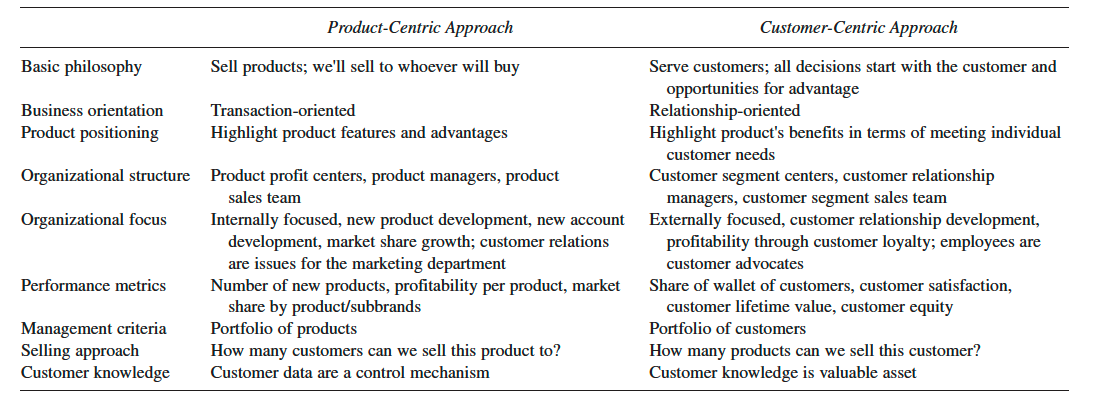
\includegraphics[scale=2, width=\textwidth]{dippa/images/ProductVsCustomer.png}
    \caption{Differencies in product-centric and customer-centric approaches by \textcite{PathToCustomerCentricity:2006}.}
    \label{fig:productvscustomer}
  \end{center}
\end{figure}

Being closer with the client means that the company have customized their offerings to individual customers. This is reported to happen for example by collecting information about their customers in order to understand buying patterns and through this the company has been able to influence the future purchase. To do so, the company also needs to view the problems from the perspective of the client and not through their own products. When company does this, they focus on satisfying customer needs and solving their problems and thus it can be said that they sell solutions. \parencite{Parniangtong:2017}

The value of trust and intimacy go hand in hand. A company must gain trust from the customers in order to maintain the relationship. When trust is earned, the goal is to create value through customer intimacy because companies want that making business with them is easy. To do so, company must show to the customer that they care about them, value their business and are aware of their needs as individual and unique customers. \parencite{Parniangtong:2017}

To gain the long-term profits from a customer-centric view, the company need to succeed in the following areas: customer acquisition, customer retention and customer development. Customer acquisition aims to get highly committed customers to be as advocates for the company by helping to look for new customers, increase the amount referrals and understand the cost as well as the value of new customer acquisition. The goal of customer retention is to lengthen the relationships between the company and the best customers as well as to lower the cost of maintaining such relationships. Lastly, customer development strives to develop customers in the direction where they would buy more products or services from the company. \parencite{Fader:2012}

\subsection{Segmentation}

In the Lean Entrepreneur by \textcite{LeanEntrepreneur:2013} highlight the fact that the \emph{who} will buy is as important as the product. To serve for a specific group of people, segmentation is needed in order to define the marketing and sales plans as well as the distribution channels to answer the needs of that specific group. If there is no segmentation done, the company do not have an understanding on who is testing the value proposition. In addition, it is impossible in the beginning to create a value proposition that fits the whole market. Instead, it should be notified that successful solutions develop over time through the early adapters.

There are many different things that suggest that customers belong to different segments. According to \textcite{LeanEntrepreneur:2013} and \textcite{BusinessModelGeneration:2010} customers belong to different segments if :
\begin{itemize}
\item They use different medias and hang out in different places, meaning that they can be reached through different distribution channels.
\item Their needs are clearly different thus it justify a distinct offer since they might be willing to pay for different things.
\item They expect different solutions and have different profitabilities.
\item Methods for selling are not the same.
\end{itemize}
The main takeaway from here is, that people might and will use the same product in different ways and it is as important to design how to market and sell the product as it is to design the actual product for their needs. And to do so, it is crucial that the company knows and understands the customers.

Another important aspect of customer segmentation is to design the value proposition. \textcite{BusinessModelGeneration:2010} states that value propositions describes the value for a customer through various elements which fill the needs of the customers. To help creating the value proposition these aspect can be for example newness of the need which is usually related to the technology, price meaning that the similar value is offered in a lower price which fills the needs of price-sensitive customers or cost which promises to reduce the costs with the help of the provided service.

One way to do segmentation is to first create a description of a customer, persona.



\subsection{Customer Journey Maps}

Based on \textcite{Kalbach:2016} operational efficiency of a company is thought as more important than their customer satisfaction. To turn this situation around, alignment diagrams can be used to help organizations to think how their business fit to the lives of customers. Alignment diagrams present the interactions between a customer and an organization in a storytelling way. Additionally, the diagrams offer a way to show both sides of value creation since they help organizations to visualize the strategy as well as they help to design experiences. \parencite{Kalbach:2016}

Alignment diagrams are beneficial because they build empathy, provide a big picture, break silos in organizations, help focusing and point where improvements and innovations can be made. Understanding better people's thoughts and feelings through alignment diagrams build empathy which allows an organization to learn about their customers and real-world human conditions. With the alignment diagrams it is possible to share the understanding and provide a big picture in organizations because the actions become more consistent and the decision making is influenced by the diagrams. \parencite{Kalbach:2016}

Because the alignment diagrams allows to map the customer experiences across different organization departments, it is possible to break down silos. In addition they help organizations to focus because alignment diagrams match the outward-facing activities with inward-facing activities. Lastly, the alignment diagrams reveal opportunities for improvements and growth because the presentation of the information allows it to be understood without middlemen. \parencite{Kalbach:2016}

According to \textcite{Kalbach:2016} the value in mapping experiences becomes from the fact that it allows to discover innovative ways to make interactions better. Moreover, the whole design of the system is then easier to make coherent.

Customer journey maps CJMs are type of alignment diagrams and \textcite{Kalbach:2016} defines customer journey maps to be visualizations about a customer's experiences and usually they illustrate how customers make a choice for example a decision to buy a service. So, customer journey maps present the steps the customers take while engaging with the company through different touchpoints \parencite{Richardson:2010}.

More precisely, CJM's present the interactions in a chronological way including for example customer's actions, thoughts, feelings and pain points. From the organizational view point the CJM's present the roles and departments who are part of creating the experience for the customer. \parencite{Kalbach:2016}

Nowadays, multi-channel shopping has become a standard in the consumer decision-making process because of mobile technologies and social media. 

Customer Buying Behavior Process Model
path-to-purchase modeling
f customer decision processes and
experience when buying products

\section{Service selling}

To deliver the value proposition and sell the service for customers the company needs to think the channels which are used to reach the customers. These channels offers touch points for creating customer experience and the channel phases can be divided into awareness, evaluation, purchase, delivery and after sales. In order to design the way to reach the customers it is important to think how they are reached now, what works and how do the company wants to reach them. \parencite{BusinessModelGeneration:2010} Customer journey maps offers a way to design such channel and are presented later in this chapter.

In business to customer ecosystem \textcite{MarketingPlans:2016} list methods for marketing products. These methods are personal selling, direct mail and email, retail outlets and and brands. In personal selling the products are usually difficult to sell meaning that the value is difficult to explain, highly profitable and commodity items meaning that the differentiation is only happening for example during the sales process. Even though personal selling is an effective way to sell since the customer is engaged in the sales process itself, it is not a cheap way to make sales happen.

Direct mail and email allows the company to target specific types of customers with lower cost compared to personal selling even though the direct contact is made. Customers can receive for example offers and catalogues via direct mail and email. However, the downside of direct mail is that the response rate is low and some might feel they lose the personal contact. \parencite{MarketingPlans:2016}

In consumer products, it is normal that the suppliers have their offering distributed by retailers with whom they have good relations and who have decent organizations for retail because of the customers are dispersal. One of the most important thing in creating and maintaining relationships with customers is to have a strong brand. Brand allows for customers to match their values, aspirations and lifestyle with the brand and through this the company might not need that much of a personal contact with the customers since they are attracted to the brand itself. \parencite{MarketingPlans:2016}

\textcite{MarketingPlans:2016} highlights the product promise to be an important aspect in service marketing compared to product marketing because the value of the service is assessed only on consumption. So, buying a service requires trust and relationship between the customer and the supplier. In addition, evaluating an offer about service is hard and it requires tangible evidence of the quality.






